\documentclass[french]{beamer}

\usepackage[utf8]{inputenc}
\usepackage[T1]{fontenc}
\usepackage{verbatim}
\usepackage{url}
\usepackage{booktabs}       % professional-quality tables
\usepackage{amsfonts}       % blackboard math symbols
\usepackage{nicefrac}       % compact symbols for 1/2, etc.
%\usepackage{microtype}      % microtypography
\usepackage{amsmath}
\usepackage{caption}
\usepackage[ruled,vlined]{algorithm2e}
\usepackage{graphicx}

\usetheme{Warsaw}


\begin{document}


		\begin{frame}
		\frametitle{Bla}
		\begin{center}
		\Large{\textbf{Breaking News Bandit}}
		\vspace{20pt}
		\end{center}
	
	\begin{center}
	Achille Aknin \& Alban Pierre

	20th January 2017
	\end{center}
		\end{frame}
	

	\section{Introduction}
	\begin{frame}
	\frametitle{Introduction}
	
	\begin{abstract}
		Multi-armed bandits are very common problems, studied with many different approachs.
		Besides, it is also derived in many ways, such as adversarial bandit, non-stationary bandit or distributed bandit.
		Here we focus on a variation called
		Breaking News Multi-armed bandit, when one arm can have suddenly a high reward: this arm stays hot for a time before it comes back to normal.
		In this report, we describe a model of such Multi-armed Bandits and then expose some algorithms to maximize the rewards
		on Breaking News Multi-armed Bandits, before testing it on our model.
	\end{abstract}
	
	\end{frame}
	
	\begin{frame}
		
		\tableofcontents[]
	\end{frame}
	
	\begin{frame}
	\frametitle{Introduction}
	
	The Multi-armed Bandit (MAB) is a very important problem in the field of Reinforcement Learning.
	Usually, it is modeled as a set of $A$ actions, called arms, that can be used at any time,
	and sending a reward to the user when he uses it. The general purpose is to create an algorithm that
	maximizes the reward over time without knowing the law controlling the rewards obtained
	for each arm.
	
	In this report, we focus on a specific type of MAB problem, called Breaking News MAB,
	where at each point of time, an arm can suddently have a higher mean reward for a short duration. The expectation can become
	very high compared to normal rewards, so, if possible, we should keep pulling the same
	arm while it is hot. When no arm is hot, the algorithm should pull each arm frequently
	in order to find a new breaking new. But during that time, the algorithm should
	also maximize the reward, because each arm does not have the same 'normal' reward.
	
	Our report is organized as follows: in the first
	section, we explain the model we used for data generation and in the second section, we recall the widely used
	Upper Confidence Bound algorithms for classic MAB problems. Then we describe
	several algorithms fitting the Breaking News MAB problem.
	Eventually, in the last section we provide more results for different problems and comparison between
	the previously exposed algorithms.
	\newline
	
	Note: the code we used in our experiments is in matlab (compatible with octave) and can be found at the address: https://github.com/alban-pierre/projet-RL-Breaking\_news\_bandit
	
	\end{frame}

	\begin{frame}
	\frametitle{Data generation}
	\section{Data generation}
	Several states per arms, with a Gaussian distribution
	\begin{itemize}
		\item At most one hot arm for a time $t$
		\item Several hot arms at the same time $t$ possible
	\end{itemize}
	
	\begin{figure}[h]
			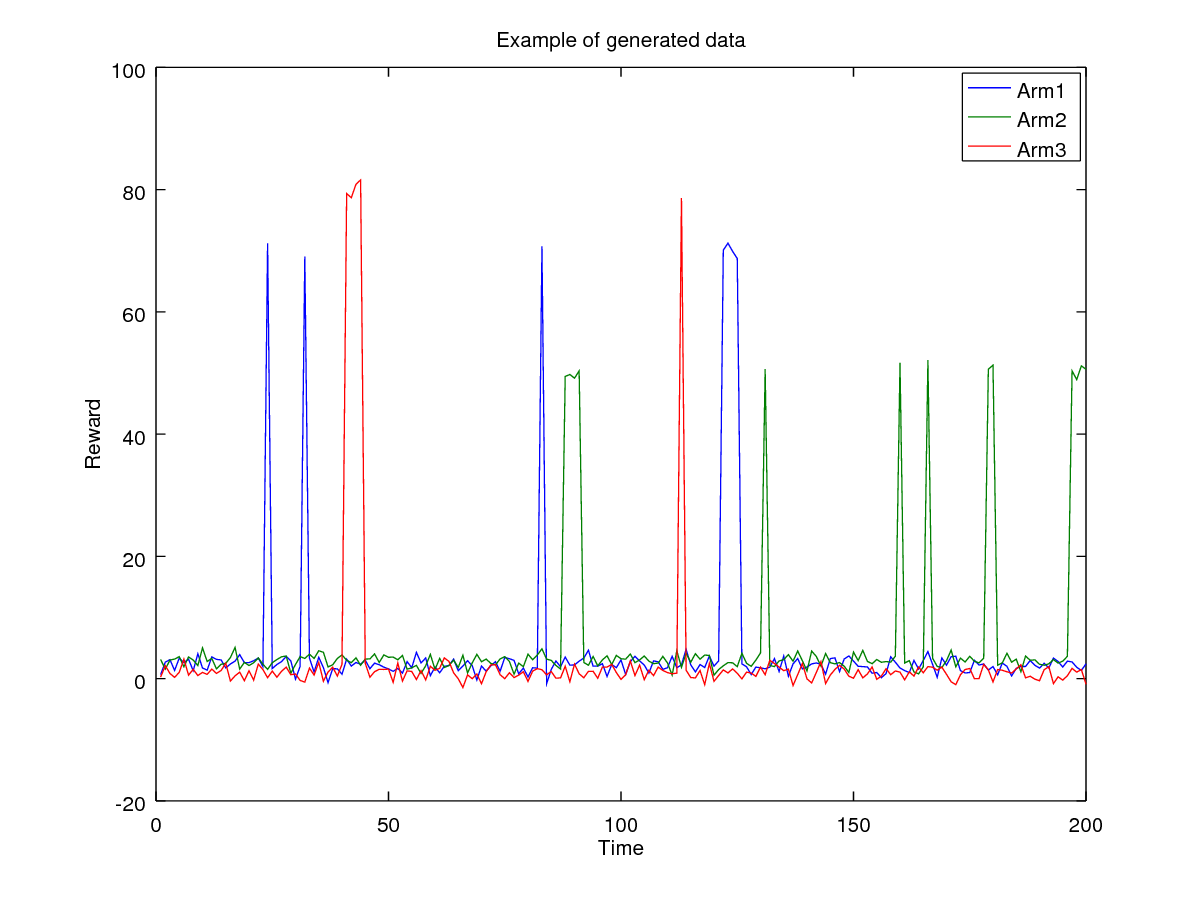
\includegraphics[width=0.7\linewidth]{generated_data_one.png}
			%\caption{Example of generated data}

		\label{fig:f}
	\end{figure}
	
	
\end{frame}

\begin{frame}
	\frametitle{Upper Confidence Bound Algorithm}
	
	In this section, we recall the widely used Upper Confidence Bound (UCB) Algorithm,
	as described in [1],
	that seeks to optimize the reward in the case of a regular MAB problem. The main
	idea is to compute an expected mean for each arm $\hat\mu_a(t)$, upper bounding it
	by a confidence on the mean being high for arms that haven't been drawn often. We
	then draw the arm with the highest upper bound.
	This way we make sure that every arm is used from time to time.
	\begin{equation*}
	a^* = argmax_{a} \Big(\hat\mu_a(t) + \sqrt{\frac{log(t)}{2N_a(t)}}\Big)
	\end{equation*}

%	\begin{algorithm}
%		\caption{UCB Algorithm}
%		\For{$i=1:T_{max}$}{
%			Compute $a^* = argmax_{a} \Big(\hat\mu_a(t) + \sqrt{\frac{log(t)}{2N_a(t)}}\Big)$\;
%			Draw arm $a^*$ and receive reward $r(t)$\;
%			Update $\hat\mu_{a^*}(t+1) = \frac{N_{a^*}(t)\times \hat\mu_{a^*}(t) + r(t)}{N_{a^*}(t)+1}$\;
%			Update $N_{a^*} = N_{a^*}+1$\;
%		}
%	\end{algorithm}
	
	This algorithm is meant to be used on a regular MAB, with reward functions that do not
	change over time. In this report, we would like to take advantage of the fact that
	we know the MAB follows the model described in last section. Most of the algorithms
	we present on next section are based on the UCB algorithm, and adapted to fit our model
	of Breaking News Bandit.

	
\end{frame}

\begin{frame}
	\frametitle{Exact probabilities inference with Gaussian Mixture}
	\section{Breaking News MAB Algorithms}
	\subsection{Exact probabilities inference with Gaussian Mixture}
	
	Tries to be mathematically exact.
	\begin{itemize}
		\item Gaussian mixture (EM algorithm)
		\item Computes probabilities of each state from an observed reward
		\item Computes transition probabilities (gradient descent)
	\newline
	\end{itemize}
	
	$\rightarrow$ Very long to compute
	
	$\rightarrow$ Parameters very sensible to little changes
	
	$\rightarrow$ Takes too much time to get stable parameters
	
\end{frame}

\begin{frame}
	\frametitle{Intuitions for Breaking News Bandit algorithms}
	\begin{figure}[h]
		\begin{center}
			%\framebox[4.0in]{$\;$}
			%\fbox{\rule[-.5cm]{0cm}{4cm} \rule[-.5cm]{4cm}{0cm}}
			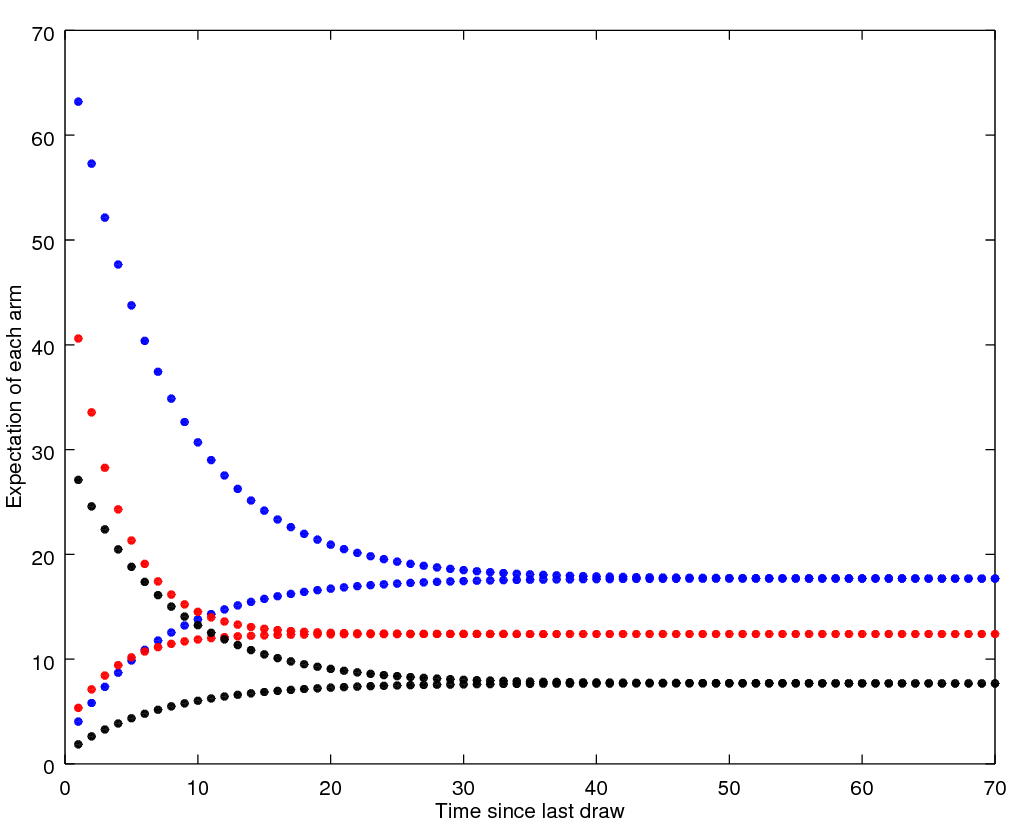
\includegraphics[width=0.78\textwidth]{expectations.png}
		\end{center}
		\caption{Expectation of each arm as a function of time since the last draw}
	\end{figure}
	
\end{frame}

\begin{frame}
	\frametitle{Nearest Neighbors Upper Confidence Bound Algorithms}
	
	\subsection{Nearest Neighbors Upper Confidence Bound Algorithms}
	
	\begin{itemize}
		\item Monte-Carlo estimation
		\item Embeds all previous rewards in a space (Last reward of the arm; Time since last draw) with some convenient deformations.
		\item For a new point, it computes the average expectation of neighbors
	\end{itemize}
	
\end{frame}

\begin{frame}
	\frametitle{K-Nearest Neighbors Long Term Expectation}
	
	\subsection{K-Nearest Neighbors Long Term Expectation}
	
	Tries to have a long term strategy instead of a greedy choose of next draw.
	\newline
	
	It pulls arms according to the $n$ future rewards (with a decay rate)
	
\end{frame}

\begin{frame}
	\frametitle{UCB\_Var}
	
	\subsection{UCB\_Var}
	
	In this section, we describe an algorithm based on the UCB algorithm and on an estimation of the maximal
	value that an arm can reach when it is not hot, and use this estimation to detect when the
	arm is hot. Our purpose is then to estimate from a sequence of samples on a given arm $a$ the range
	of values we expect the next sample to be in. We will then exploit the mean $\hat\mu_a(t)$ and variance $\hat\sigma_a(t)$
	estimated from the previous samples and consider that if an arm stays in its initial
	state, the reward drawn $r$ should be in the range $r \in [\hat\mu_a(t)-\hat\sigma_a(t), \hat\mu_a(t)+\hat\sigma_a(t)]$.
	
	To take into account the uncertainty on both the mean and the range we might have,
	we will add a term decreasing with the number of sample rewards we have on the arm $a$:
	\begin{equation}\label{UCB-var-bound}
	r \in \Big[\hat\mu_a(t)-\hat\sigma_a(t)-\sqrt{\frac{1}{2N_a(t)}}, \hat\mu_a(t)+\hat\sigma_a(t)+\sqrt{\frac{1}{2N_a(t)}}\Big]
	\end{equation}
	
	The algorithm is then as follows: we proceed as in the UCB algorithm, and if at
	some time $t$ we draw a sample from an arm and the reward obtained $r(t)$ is higher than the upper bound
	in Eq.~\ref{UCB-var-bound}, we then consider that this arm is in a hot state.
	We temporarily forget the samples we've seen for this arm, and continue
	with $r(t)$ as the only reward observed so far for arm $a$. This has the effect
	of having a bigger mean $\hat\mu(t+1) = r(t)$ and having $N_a(t+1) = 1$, making this arm more suceptible
	to be drawn next time. If at some time $t'$, we observe a reward $r(t')$ lower
	than the lower bound in Eq.~\ref{UCB-var-bound}, we then consider that this arm has
	left the hot state, and proceed with the samples observed before time $t$, having
	once again a smaller mean $\hat\mu(t')$.
	
	In practice, this algorithm gets quite stable and good results if we make sure,
	with some adaptations, to not keep thinking that an arm is hot when it is actually
	not. The main drawback of this algorithm is that we need to remember each
	reward observed at along, and compute its variance, and we can't avoid
	a linear operation at each step, so the algorithm has a complexity of $\mathcal{O}(N^2)$ where N
	is the number of steps.
\end{frame}

\begin{frame}
	\frametitle{UCB\_Max}
	
	\subsection{UCB\_Max}
	
	To avoid the quadratic complexity of the previous algorithm, we choose to not compute
	the actual variance $\hat\sigma_a(t)$, but instead simply remember the maximal value
	observed on each arm $M_a(t)$ (and for a hot state, the minimal value $m_a(t)$).
	At each step, we now check whether $r(t) > M_a(t)$ (or whether $r(t) < m_a(t)$ for a hot state),
	and if it is the case then we consider that arm $a$ entered the hot state (or left the hot state)
	and we reinitialise $\hat\mu_a(t)$ (or take back the old value).
	
	This algorithm does not have results as good as UCB\_Var, but it faster and only have
	a linear complexity, since computing the mean $\hat\mu_a(t)$ and the max $M_a(t)$
	can be done with a finite number of operations at each step.
	
\end{frame}

\begin{frame}
	\frametitle{Time of computation}
	
	\section{Time of computation and results}
	
	 At most one hot state, 3 arms * 2 states :
	 \newline
	 
	 
	 	\begin{tabular}{rccccc}
	 		Arms : & TS & UCB & GM & UCB\_KNN & KNN\_LONG \\
	 		Time (sec) : & 7.12 & 2.19 & 1000.5 & 25.39 & 35.85
	 	\end{tabular}
	 	\newline
	 	\newline
	 	
	 	\begin{tabular}{rcc}
	 		Arms : & UCB\_MAX & UCB\_VAR \\
	 		Time (sec) : & 3.06 & 5.37
	 	\end{tabular}
	 
\end{frame}

\begin{frame}
	\frametitle{Results (One hot arm, 3 arms * 2 states)}
	 
	\begin{figure}[h]
		\begin{center}
			%\framebox[4.0in]{$\;$}
			%\fbox{\rule[-.5cm]{0cm}{4cm} \rule[-.5cm]{4cm}{0cm}}
			\vspace{-10pt}
			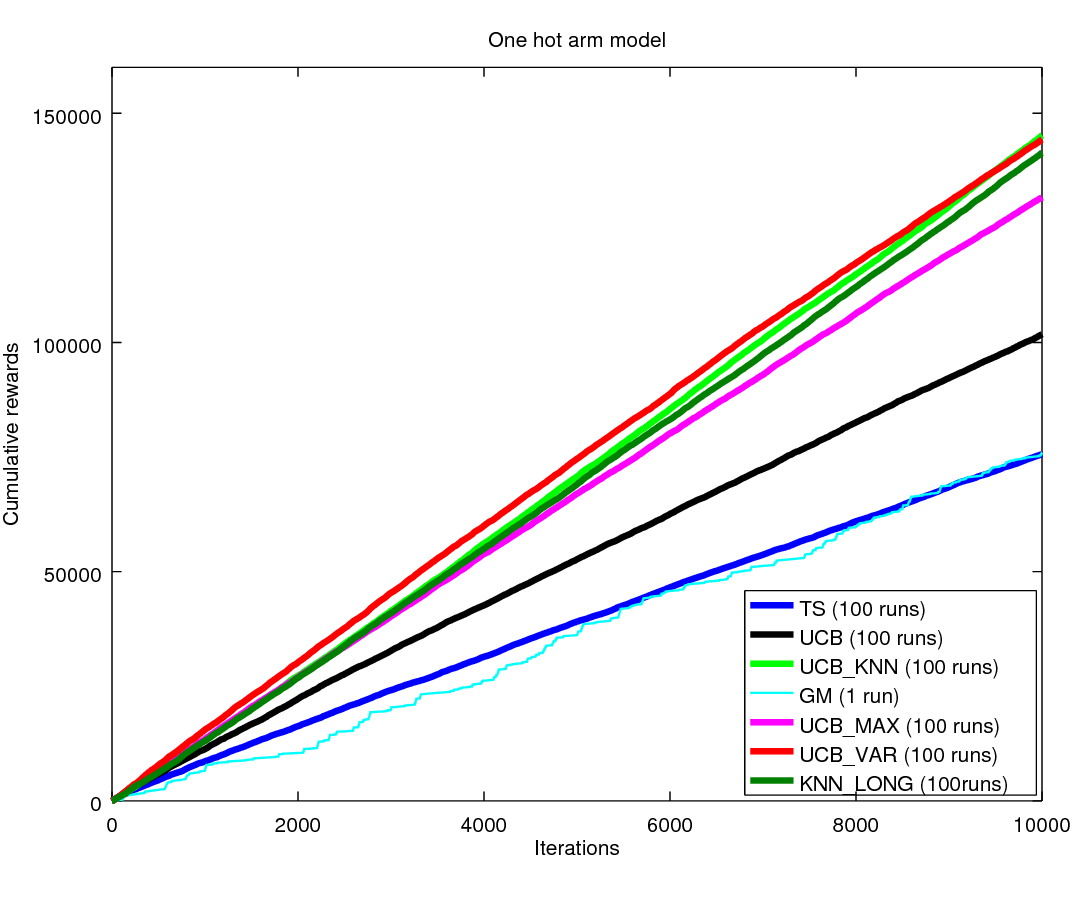
\includegraphics[width=1.05\textheight]{all_10000it.png}
			
			\vspace{-7pt}
			\scriptsize{All algorithms for 10000 iterations (3 arms * 2 states, One hot arm)}
		\end{center}
	\end{figure}
\end{frame}

\begin{frame}
	\frametitle{Results (One hot arm, 3 arms * 2 states)}	
	\begin{figure}[h]
		\begin{minipage}[b]{.49\linewidth}
			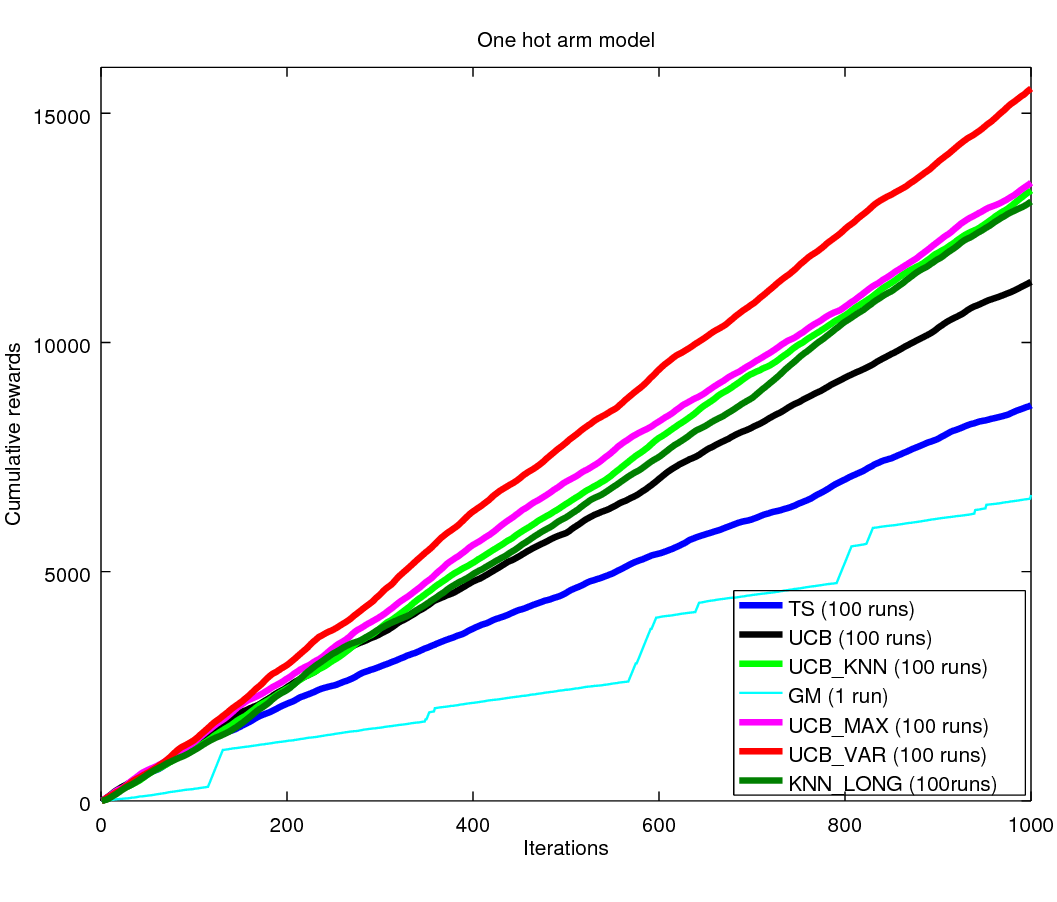
\includegraphics[width=1.0\textwidth]{begin_1000it.png}
			
			\centering{\scriptsize{1000 first iterations (3*2, one)}}
		\end{minipage}
		\hfill
		\begin{minipage}[b]{0.49\linewidth}
			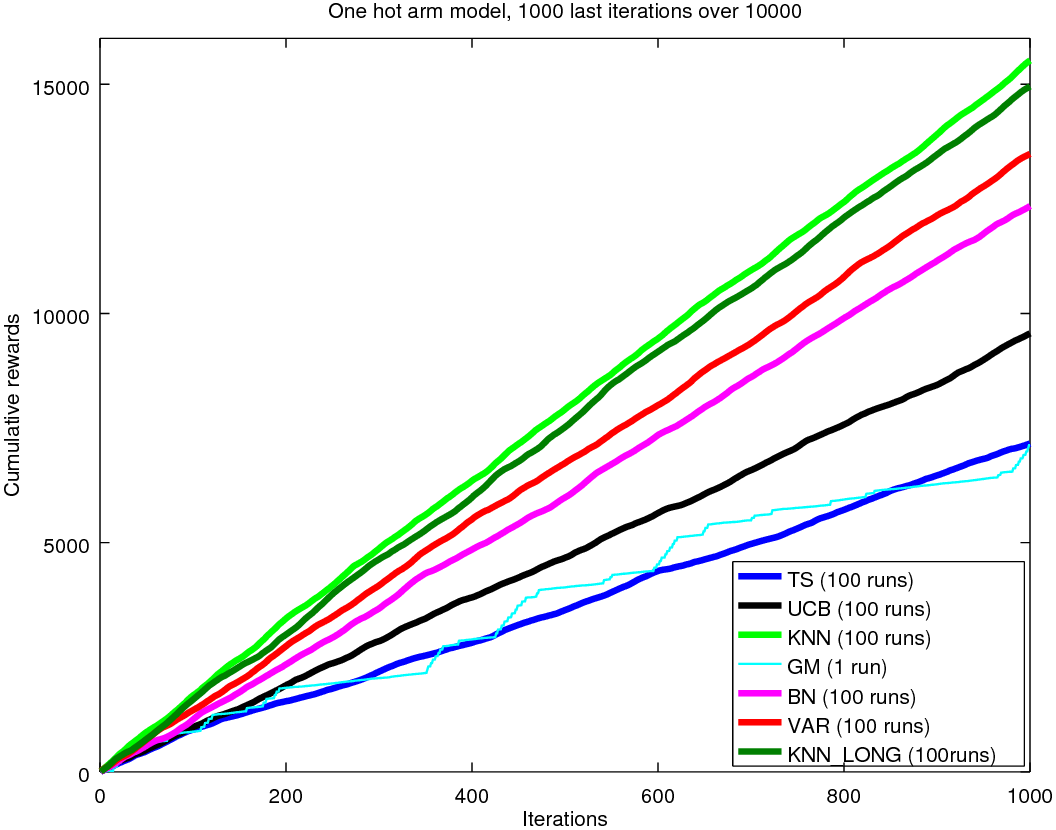
\includegraphics[width=1.0\textwidth]{last_1000it.png}
			
			\centering{\scriptsize{1000 last iterations (3*2, one)}}
		\end{minipage}
		\label{fig:f}
	\end{figure}
	
\end{frame}

\begin{frame}
	\frametitle{Results (Ona hot arm, 3 arms * 2 states)}
		
	\begin{figure}[h]
		\begin{center}
			%\framebox[4.0in]{$\;$}
			%\fbox{\rule[-.5cm]{0cm}{4cm} \rule[-.5cm]{4cm}{0cm}}
			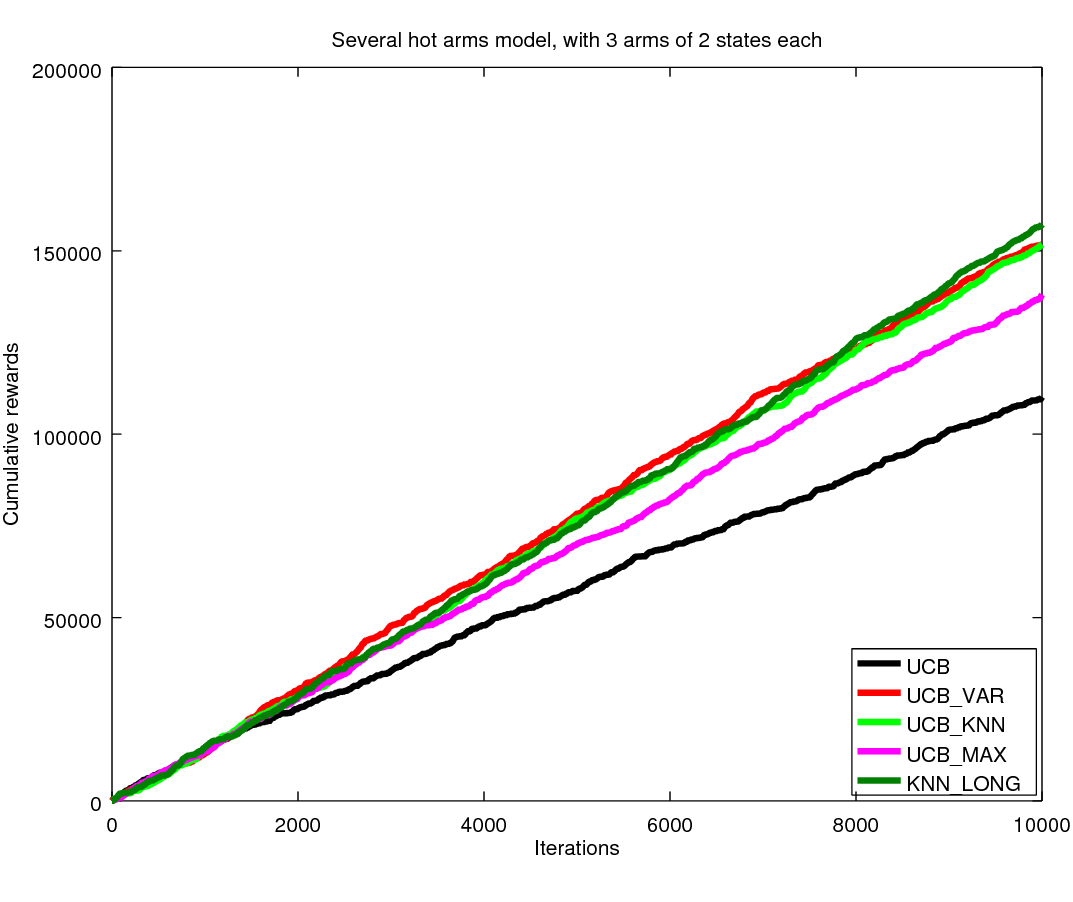
\includegraphics[width=1.0\textwidth]{all_m_10000it.png}
		\end{center}
		\caption{All algorithms for 10000 iterations (3 arms * 2 states, several hot arms)}
	\end{figure}
	
	\begin{figure}[h]
		\begin{minipage}[b]{.49\linewidth}
			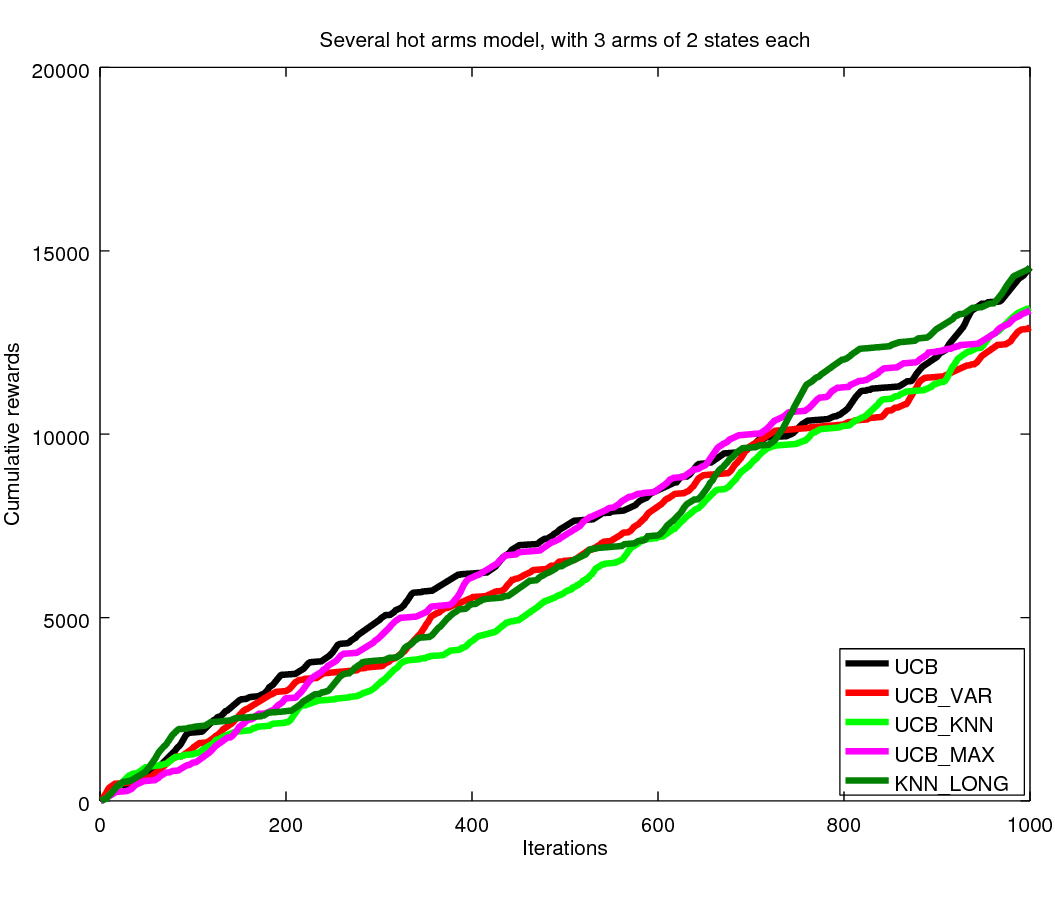
\includegraphics[width=1.0\textwidth]{begin_m_1000it.png}
			\caption{1000 first iterations (3*2, several)}
		\end{minipage}
		\hfill
		\begin{minipage}[b]{0.49\linewidth}
			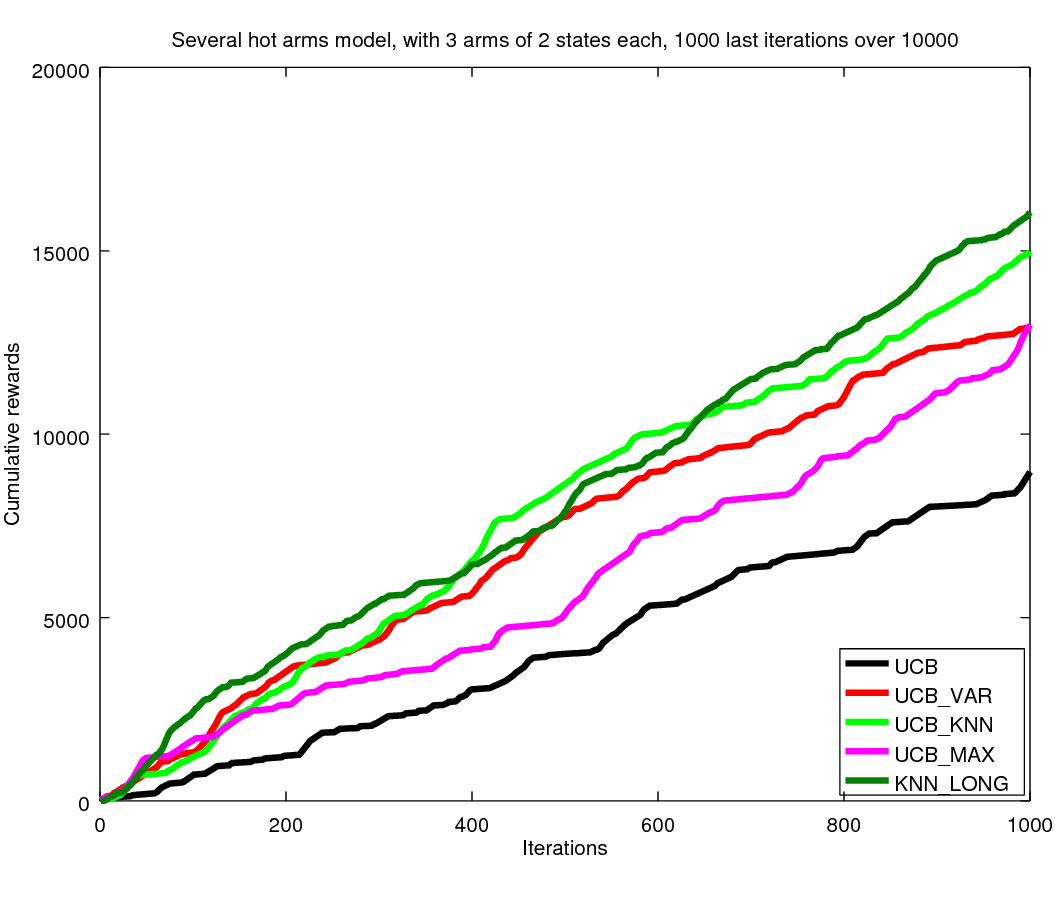
\includegraphics[width=1.0\textwidth]{last_m_1000it.png}
			\caption{1000 last iterations (3*2, several)}
		\end{minipage}
		\label{fig:f}
	\end{figure}
	
	We observe quite the same things except for KNN\_LONG : this algorithm sometimes tries different arms while they were on a hot arm with a comparatively low hot reward. The other algorithms keep hitting the same arm when it is hot, so they don't see the difference from the case where there are at most one hot arm.
	
	\clearpage
	Then we tried with 5 arms with 3 states each (with one hot arm at most, 10 runs each) :
	
	\begin{figure}[h]
		\begin{center}
			%\framebox[4.0in]{$\;$}
			%\fbox{\rule[-.5cm]{0cm}{4cm} \rule[-.5cm]{4cm}{0cm}}
			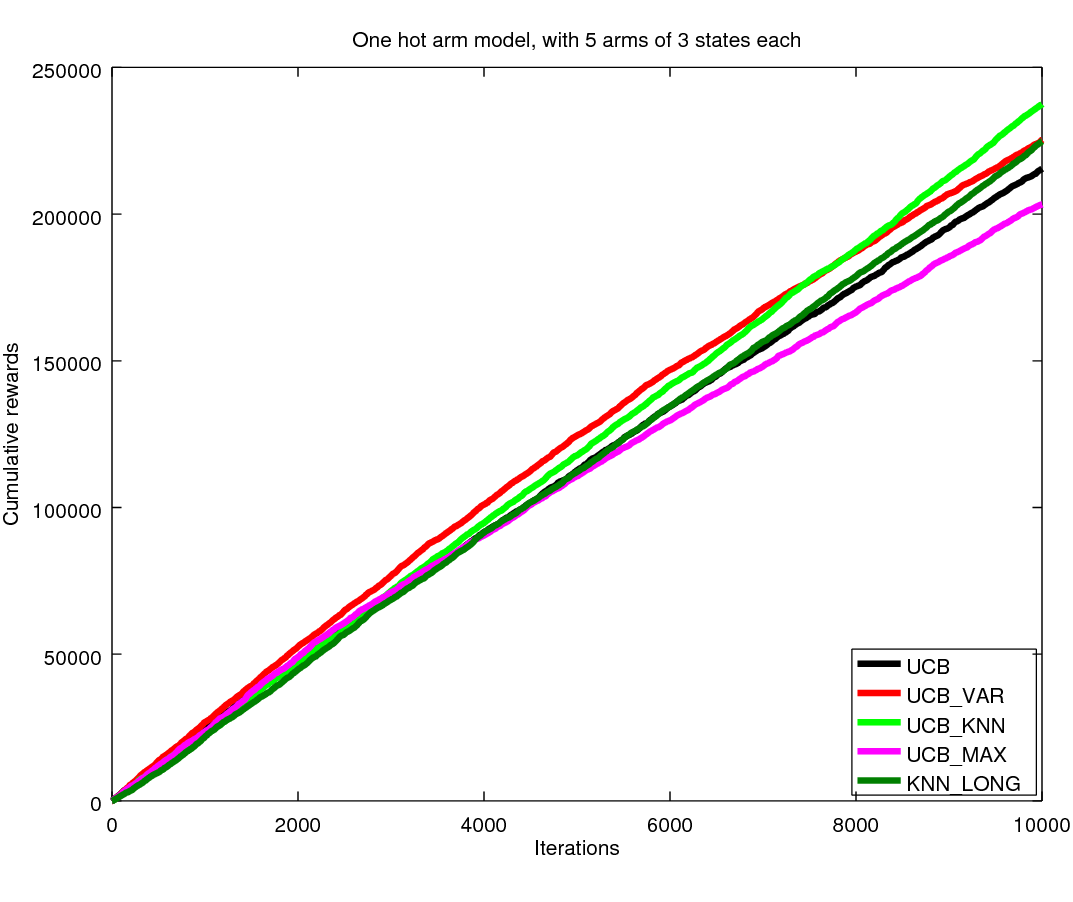
\includegraphics[width=1.0\textwidth]{all_s_10000it.png}
		\end{center}
		\caption{All algorithms for 10000 iterations (5 arms * 3 states, at most one hot arm)}
	\end{figure}
	
	\begin{figure}[h]
		\begin{minipage}[b]{.49\linewidth}
			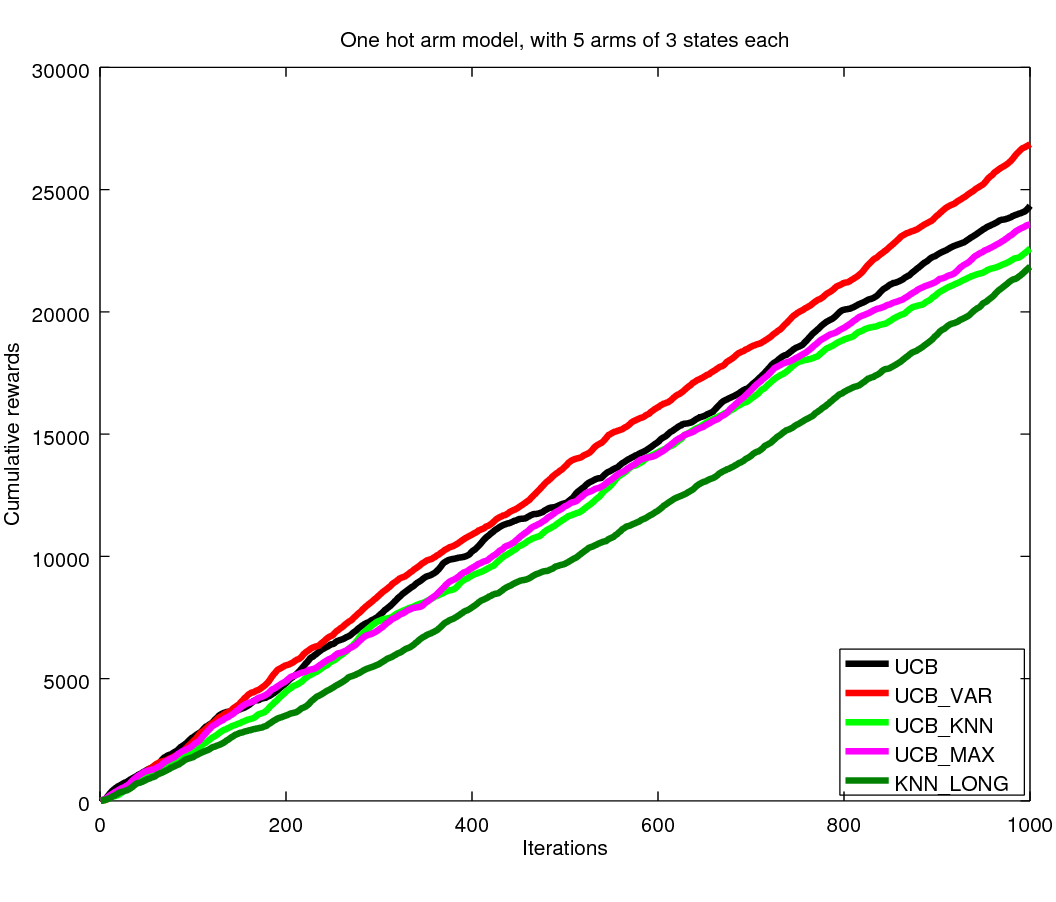
\includegraphics[width=1.0\textwidth]{begin_s_1000it.png}
			\caption{1000 first iterations (5*3, one)}
		\end{minipage}
		\hfill
		\begin{minipage}[b]{0.49\linewidth}
			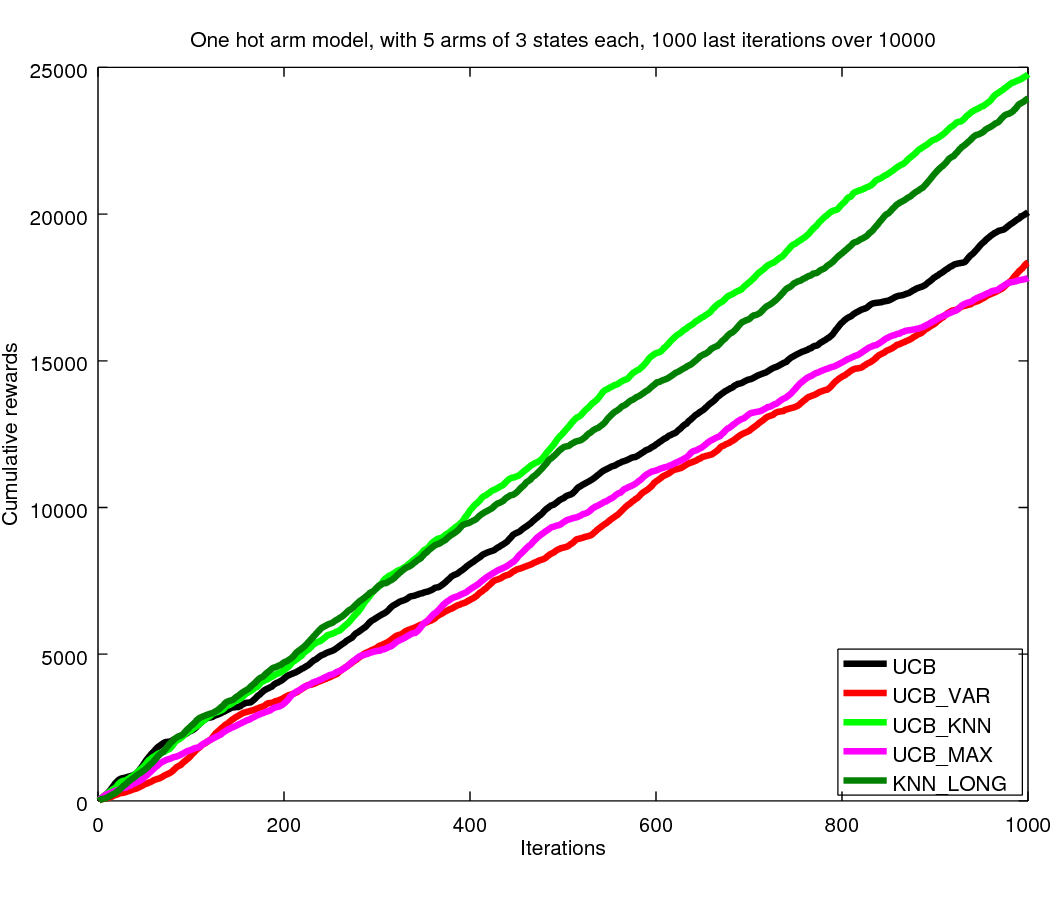
\includegraphics[width=1.0\textwidth]{last_s_1000it.png}
			\caption{1000 last iterations (5*3, one)}
		\end{minipage}
		\label{fig:f}
	\end{figure}
	
	We observe that the UCB algorithm performs better, indeed as there are more arms, it explores more so it finds more hot states and high rewards.
	
	\clearpage
	Eventually we tried the same version with several hot arms (5 runs each) :
	
	\begin{figure}[h]
		\begin{center}
			%\framebox[4.0in]{$\;$}
			%\fbox{\rule[-.5cm]{0cm}{4cm} \rule[-.5cm]{4cm}{0cm}}
			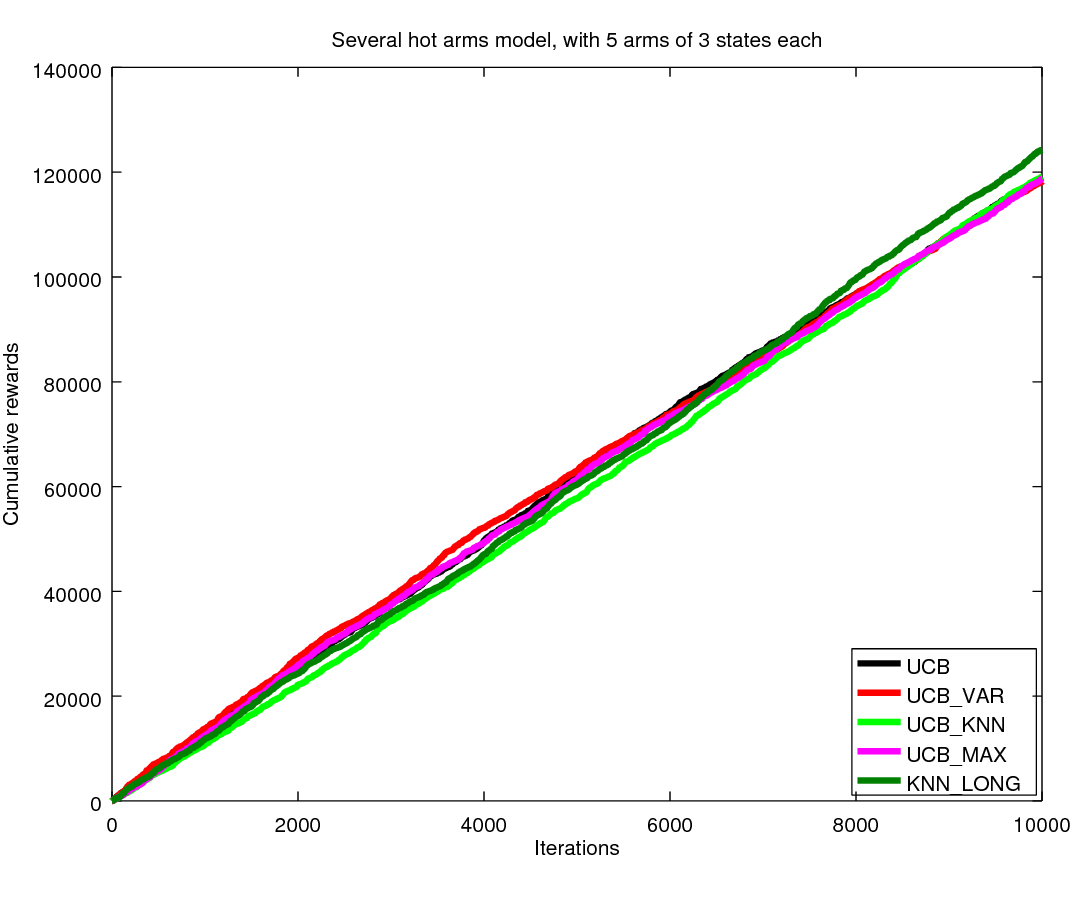
\includegraphics[width=1.0\textwidth]{all_ms_10000it.png}
		\end{center}
		\caption{All algorithms for 10000 iterations (5 arms * 3 states, several hot arms)}
	\end{figure}
	
	\begin{figure}[h]
		\begin{minipage}[b]{.49\linewidth}
			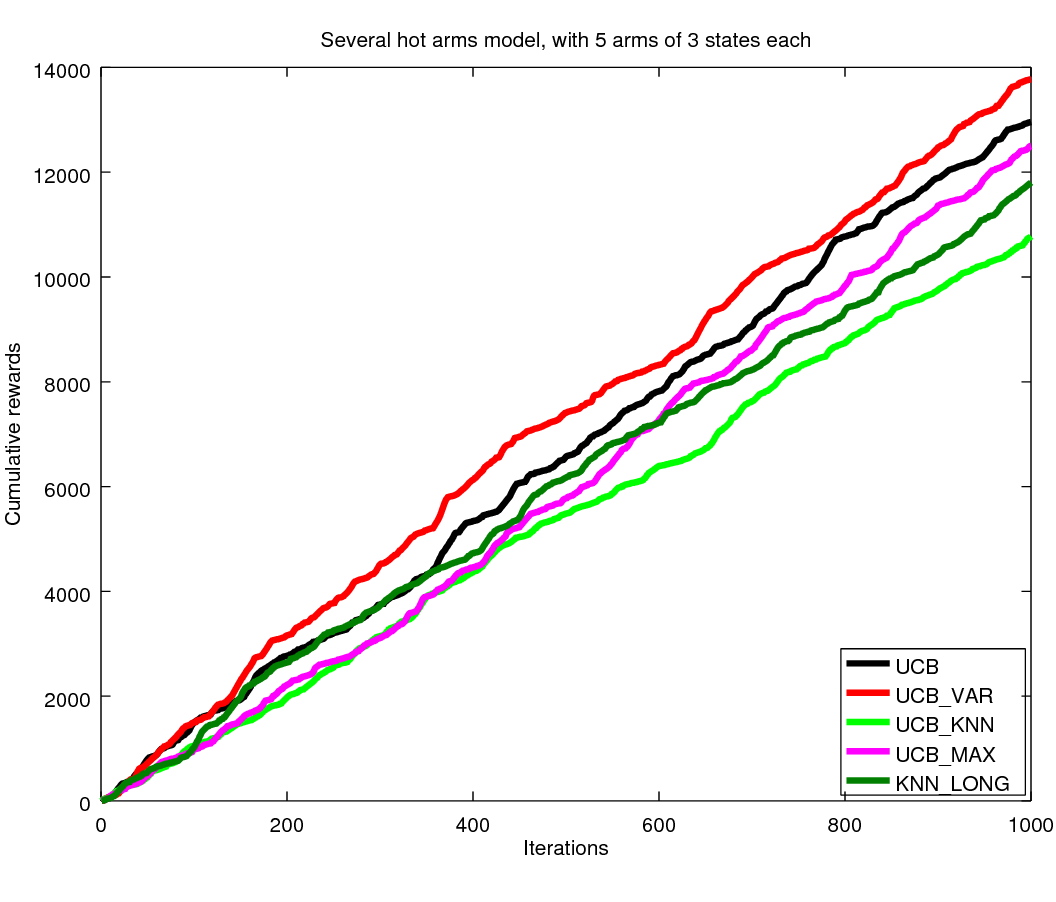
\includegraphics[width=1.0\textwidth]{begin_ms_1000it.png}
			\caption{1000 first iterations (5*3, several)}
		\end{minipage}
		\hfill
		\begin{minipage}[b]{0.49\linewidth}
			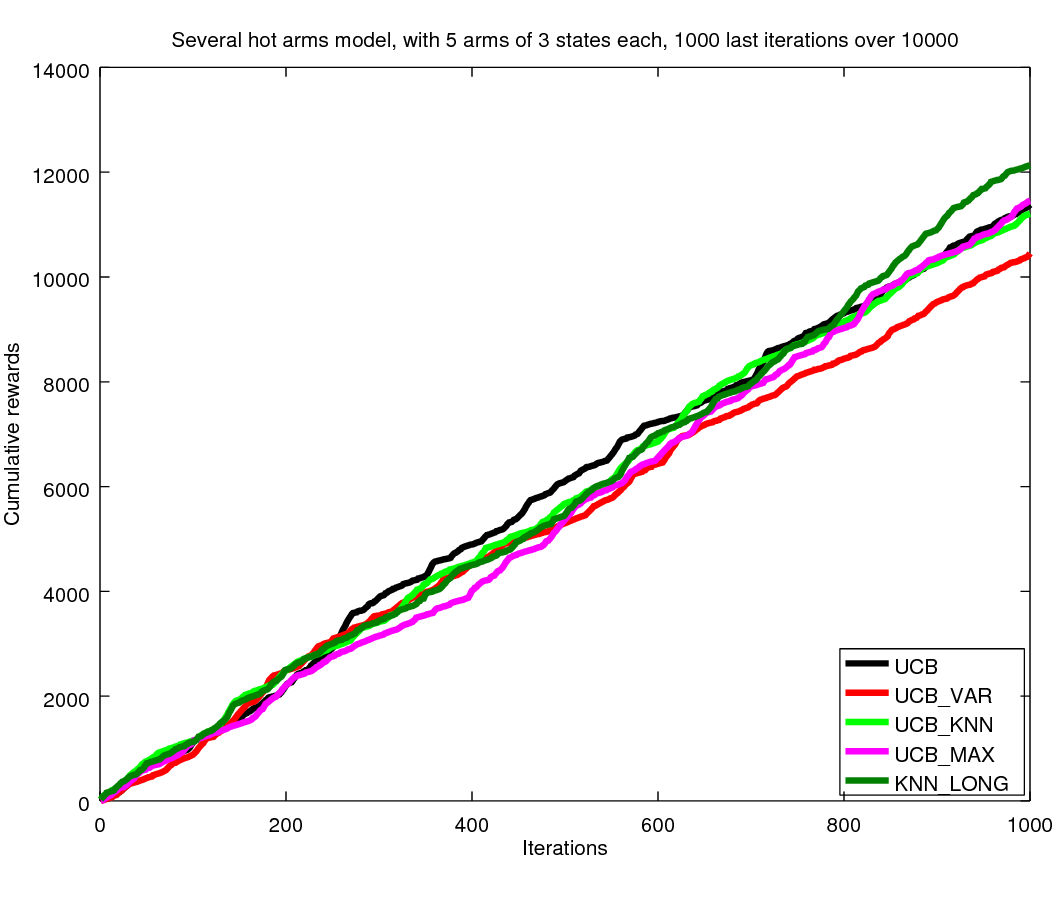
\includegraphics[width=1.0\textwidth]{last_ms_1000it.png}
			\caption{1000 last iterations (5*3, several)}
		\end{minipage}
		\label{fig:f}
	\end{figure}
	
	Here again the KNN\_LONG algorithm takes advantage for having a long term expectation calculation.
	
	\clearpage
\end{frame}

\begin{frame}
	\frametitle{Conclusion}
	
	\section{Conclusion}
	
	We have shown that for the special case of multi armed bandit problems where an arm can become hot and have a big reward temporarily, classical algorithms like Thompson Sampling or Upper Confidence Bound miss high rewards as they explore less and less across time.
	
	To tackle this problem, we have tried to use the variance and the maximum of previous rewards of an arm to estimate when an arm is hot, then pulling always the hot arm. This lead to good results, but they don't improve over time. We have also used an algorithm that uses a Monte-Carlo approximation of expectation, it performs better in the end but it has a very long initialization phase.
	
	In the case where many hot arms can become hot simultaneously, we have shown that an algorithm that pulls arms according to the maximum of its expectation over many following draws can perform better than greedy algorithms over the next draw. But it has still difficulties to get a significantly better result, and it could be interesting for further research to develop an algorithm that computes some sort of fixed point - just like figure 2 but with a reward over many following draws - to get the best greedy policy.
	
\end{frame}

\begin{frame}
	\frametitle{references}
	
	
	\small{
		\begin{itemize}
		\item [1] Auer, P., Cesa-Bianchi, N., \& Fischer, P. (2002). Finite-time analysis of the multiarmed bandit problem. Machine learning, 47(2-3), 235-256.
		
		\item [2] Agrawal, S., \& Goyal, N. (2012, June). Analysis of Thompson Sampling for the Multi-armed Bandit Problem. In COLT (pp. 39-1).
		\end{itemize}
	}
\end{frame}
	
	\begin{frame}
	\frametitle{Remerciements}
	
	Thank you for your attention !
	
	\end{frame}

\end{document}






